\documentclass[10pt,twocolumn]{article}

\usepackage[letterpaper,top=0.85in,bottom=0.85in,left=0.75in,right=0.75in,columnsep=0.3in]{geometry}
\usepackage[utf8]{inputenc}
\usepackage[expansion=false]{microtype}
\usepackage{amsmath,amssymb}
\usepackage{booktabs}
\usepackage{graphicx}
\usepackage{xcolor}
\usepackage{enumitem}
\usepackage{caption}
\usepackage[linesnumbered,ruled,vlined,noend]{algorithm2e}
\usepackage{tikz}
\usetikzlibrary{arrows.meta,positioning,fit,calc,shapes.geometric,backgrounds}
\usepackage{pgfplots}
\pgfplotsset{compat=1.17}
\usepackage[colorlinks=true,linkcolor=blue!50!black,citecolor=blue!50!black,urlcolor=blue!50!black]{hyperref}

\emergencystretch=2em
\setlength{\parskip}{0pt}
\setlist{nosep,leftmargin=1.4em}
\captionsetup{font=small,labelfont=bf,labelsep=colon}
\setlength{\abovecaptionskip}{4pt}

% --- macros -------------------------------------------------------------
\newcommand{\statis}{\textsc{Statis}}
\newcommand{\sys}[1]{\texttt{\detokenize{#1}}}
\newcommand{\pending}[1]{\textcolor{red!70!black}{[PENDING: #1]}}
\newcommand{\yes}{\checkmark}
\newcommand{\no}{$\times$}
\DeclareMathOperator{\Warp}{warp}

\definecolor{supc}{RGB}{225,236,250}
\definecolor{chic}{RGB}{252,236,215}
\definecolor{kerc}{RGB}{232,232,232}
\definecolor{accent}{RGB}{31,78,140}
\definecolor{warn}{RGB}{190,60,40}

\SetKwComment{Comment}{$\triangleright$\ }{}
\SetCommentSty{textit}
\SetAlFnt{\small}
\SetAlCapFnt{\small}
\SetAlCapNameFnt{\small}

\begin{document}

\twocolumn[{%
\begin{center}
{\LARGE\bfseries Statis: High-Performance Seed-Deterministic\\[2pt] Userspace Supervision for Unmodified Linux Binaries\par}
\vspace{1.3em}
{\large\bfseries Siddid Pandey}\\[2pt]
Qvost\par
\vspace{1.2em}
\end{center}
\begin{center}
\begin{minipage}{0.88\textwidth}
\begin{center}{\bfseries Abstract}\end{center}\vspace{-4pt}
\small\noindent\hspace{1.5em}%
A Linux process is nondeterministic for reasons that have nothing to do with its own logic: it reads a clock, executes \sys{rdtsc}, sleeps, races its threads, and receives whatever errors the network chooses to deliver. Existing tools either record everything that happened (and store gigabytes to replay it) or rebuild a deterministic container around the program. We ask whether a single \emph{userspace} supervisor, with no kernel module and no recompilation, can make an unmodified binary a pure function of one integer seed. We introduce \statis, a supervisor that takes control of every source of nondeterminism a program can observe. It blinds the vDSO by rewriting \sys{AT_SYSINFO_EHDR} to \sys{AT_IGNORE} in the ELF auxiliary vector at every \sys{execve}, so libc must issue real, interceptable system calls. It emulates \sys{rdtsc}/\sys{rdtscp} through \sys{PR_TSC_SIGSEGV} and a virtual clock. It replaces wall-clock waiting with a min-heap time wheel, so an idle process tree warps past \sys{nanosleep}, \sys{clock_nanosleep}, \sys{epoll_wait} and \sys{poll}: a 10\,s sleep completes in 18\,ms and a 15\,s \sys{epoll_wait} in 17\,ms, over 500$\times$ faster than wall clock. A userspace futex manager and PMU-driven instruction quanta make multithreaded schedules a function of the seed; a ChaCha20 stream derived from the same seed injects reproducible system-call errors. Replay needs only a compact, little-endian trace of kilobytes (versus gigabytes for \sys{rr}), checked by \emph{semantic} argument matching so that stack-pointer shifts do not raise false divergences. \statis{} is open source.
\end{minipage}
\end{center}
\vspace{0.8em}
}]

%=========================================================================
\section{Introduction}
%=========================================================================
Debugging a distributed system, a flaky test, or a concurrency bug is hard because the failing execution cannot be summoned on demand. The program is not the only author of its behavior. The kernel contributes the time of day, the interleaving of threads, the readiness of file descriptors, and the occasional \sys{ECONNRESET}; the CPU contributes a cycle counter that any unprivileged instruction can read. Two runs of the same binary on the same input diverge, and the bug disappears under the debugger.

Two families of tools attack this. \emph{Record-and-replay} systems such as \sys{rr}~\cite{rr} log every nondeterministic input of one run and re-execute it faithfully; the price is a recording that grows with the program's activity and a dependence on hardware performance counters. \emph{Deterministic containers} such as DetTrace~\cite{dettrace} and Hermit~\cite{hermit} instead rebuild the execution environment so that nondeterminism is removed (or controlled by a seed) at the source, with no recording needed. Our work sits in the second family, and asks how little machinery that takes.

We observe that, on Linux/x86-64, \emph{every} observable source of nondeterminism crosses one of four boundaries: a system call, a trapped instruction, a thread-scheduling decision, or the ELF auxiliary vector that tells libc where fast paths live. A supervisor that owns all four can turn the program into a deterministic function of a seed, without touching the kernel or the binary. \statis{} is that supervisor.

\begin{figure*}[t]
\centering
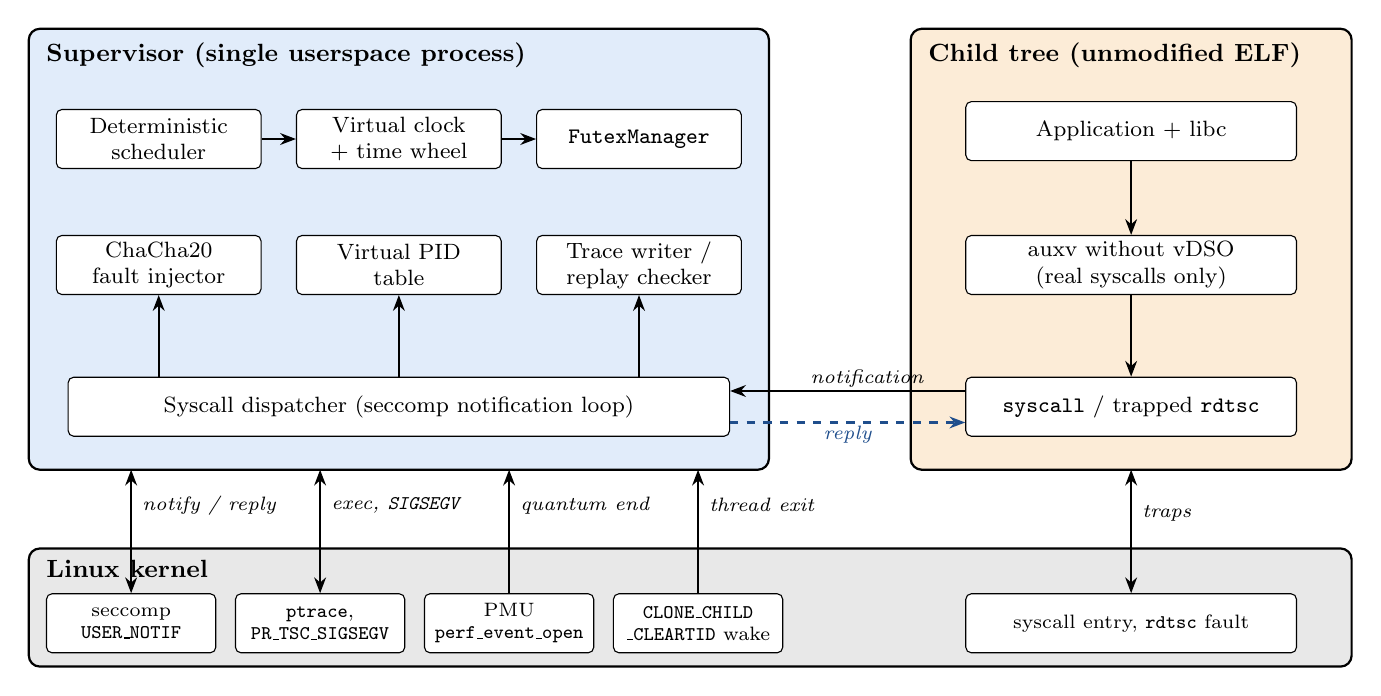
\begin{tikzpicture}[font=\footnotesize,
  box/.style={draw,rounded corners=2pt,align=center,minimum height=7.5mm,minimum width=2.6cm,inner sep=2pt,fill=white},
  frame/.style={draw,rounded corners=4pt,thick},
  arr/.style={-{Stealth[length=2mm]},thick},
  darr/.style={{Stealth[length=2mm]}-{Stealth[length=2mm]},thick},
  lab/.style={font=\scriptsize\itshape,inner sep=1pt}]
% supervisor
\draw[frame,fill=supc] (0,0) rectangle (9.4,5.6);
\node[font=\small\bfseries,anchor=north west] at (0.1,5.55) {Supervisor (single userspace process)};
\node[box] (sched) at (1.65,4.2) {Deterministic\\scheduler};
\node[box] (clock) at (4.7,4.2) {Virtual clock\\+ time wheel};
\node[box] (futex) at (7.75,4.2) {\texttt{FutexManager}};
\node[box] (fault) at (1.65,2.6) {ChaCha20\\fault injector};
\node[box] (vpid)  at (4.7,2.6) {Virtual PID\\table};
\node[box] (trace) at (7.75,2.6) {Trace writer /\\replay checker};
\node[box,minimum width=8.4cm] (disp) at (4.7,0.8) {Syscall dispatcher (seccomp notification loop)};
\draw[arr] (sched)--(clock); \draw[arr] (clock)--(futex);
\foreach \n in {fault,vpid,trace}{\draw[arr] (disp.north -| \n.south) -- (\n.south);}
% child
\draw[frame,fill=chic] (11.2,0) rectangle (16.8,5.6);
\node[font=\small\bfseries,anchor=north west] at (11.3,5.55) {Child tree (unmodified ELF)};
\node[box,minimum width=4.2cm] (app) at (14.0,4.3) {Application + libc};
\node[box,minimum width=4.2cm] (aux) at (14.0,2.6) {auxv without vDSO\\(real syscalls only)};
\node[box,minimum width=4.2cm] (sc)  at (14.0,0.8) {\texttt{syscall} / trapped \texttt{rdtsc}};
\draw[arr] (app)--(aux); \draw[arr] (aux)--(sc);
\draw[arr] ([yshift=2mm]sc.west) -- node[lab,above] {notification} ([yshift=2mm]disp.east -| 9.4,0) -- ([yshift=2mm]disp.east);
\draw[arr,dashed,color=accent] ([yshift=-2mm]disp.east) -- node[lab,below] {reply} ([yshift=-2mm]sc.west);
% kernel
\draw[frame,fill=kerc] (0,-2.5) rectangle (16.8,-1.0);
\node[font=\small\bfseries,anchor=north west] at (0.1,-1.03) {Linux kernel};
\node[box,minimum width=2.15cm,font=\scriptsize] (k1) at (1.3,-1.95) {seccomp\\\texttt{USER\_NOTIF}};
\node[box,minimum width=2.15cm,font=\scriptsize] (k2) at (3.7,-1.95) {\texttt{ptrace},\\\texttt{PR\_TSC\_SIGSEGV}};
\node[box,minimum width=2.15cm,font=\scriptsize] (k3) at (6.1,-1.95) {PMU\\\texttt{perf\_event\_open}};
\node[box,minimum width=2.15cm,font=\scriptsize] (k4) at (8.5,-1.95) {\texttt{CLONE\_CHILD}\\\texttt{\_CLEARTID} wake};
\node[box,minimum width=4.2cm,font=\scriptsize] (k5) at (14.0,-1.95) {syscall entry, \texttt{rdtsc} fault};
\draw[darr] (k1.north) -- (k1.north |- 0,0) node[lab,midway,right] {};
\draw[darr] (k2.north) -- (k2.north |- 0,0);
\draw[arr] (k3.north) -- (k3.north |- 0,0);
\draw[arr] (k4.north) -- (k4.north |- 0,0);
\draw[darr] (k5.north) -- (k5.north |- 0,0);
\node[lab,anchor=west] at (1.4,-0.45) {notify / reply};
\node[lab,anchor=west] at (3.8,-0.45) {exec, \texttt{SIGSEGV}};
\node[lab,anchor=west] at (6.2,-0.45) {quantum end};
\node[lab,anchor=west] at (8.6,-0.45) {thread exit};
\node[lab,anchor=west] at (14.1,-0.55) {traps};
\end{tikzpicture}
\caption{\statis{} architecture. The child's system calls reach the supervisor's dispatcher through a seccomp user-notification listener (IPC); the dispatcher consults the virtual clock, futex manager, fault injector and virtual PID table before replying. Exec stops and \texttt{rdtsc} faults arrive through \texttt{ptrace}, PMU overflows delimit scheduling quanta, and the kernel's silent thread-exit wake is surfaced to the futex manager.}
\label{fig:arch}
\end{figure*}

\paragraph{Contributions.}
\begin{itemize}
\item \textbf{vDSO neutralization.} Rewriting \sys{AT_SYSINFO_EHDR} (type 33) to \sys{AT_IGNORE} (type 1) in the auxiliary vector at every \sys{execve}, forcing libc to issue real syscalls across \sys{exec} boundaries (\S\ref{sec:vdso}).
\item \textbf{Hardware-clock emulation and time warping.} \sys{rdtsc}/\sys{rdtscp} are virtualized through \sys{PR_TSC_SIGSEGV}, and a monotonic virtual clock with a min-heap time wheel lets idle process trees skip waiting, 10\,s in 18\,ms (\S\ref{sec:tsc}--\S\ref{sec:warp}).
\item \textbf{Seed-derived concurrency and faults.} A userspace futex manager, silent-exit detection for \sys{pthread_join}, PMU instruction quanta, and ChaCha20 error injection make threads and failures functions of one seed (\S\ref{sec:conc}--\S\ref{sec:fault}).
\item \textbf{Compact trace, semantic replay.} Kilobyte-scale little-endian traces verified by semantic argument matching (\S\ref{sec:trace}).
\item \textbf{Honest evaluation.} We state which numbers are measured and which are still pending.
\end{itemize}

%=========================================================================
\section{Design}
%=========================================================================
\subsection{Overview and determinism contract}
\statis{} launches the target as a child, installs a seccomp filter in it that returns \sys{SECCOMP_RET_USER_NOTIF} for the system calls it wants to mediate, and receives the notification file descriptor over a Unix socket (\sys{SCM_RIGHTS}). The supervisor then serves a single dispatch loop (Figure~\ref{fig:arch}). Calls the supervisor does not need to change are allowed through to the kernel; the rest are answered from supervisor state.

\paragraph{Contract.} Let $B$ be a binary, $I$ its input (arguments, environment, files), and $s$ a 64-bit seed. \statis{} aims for the following property:
\begin{equation}
\mathrm{Run}(B, I, s) = \mathrm{Run}(B, I, s)\quad\text{for every run,}
\label{eq:contract}
\end{equation}
where $\mathrm{Run}$ denotes the sequence of observable events (system calls with semantic arguments and results, and trapped-instruction results). The contract holds under a \emph{closed-world} assumption: the only nondeterminism is what \statis{} virtualizes. Inputs from outside the supervised tree (live remote peers, other host processes) are outside the contract (\S\ref{sec:limits}).

\subsection{vDSO neutralization}
\label{sec:vdso}
On x86-64, libc resolves \sys{clock_gettime}, \sys{gettimeofday}, \sys{time} and \sys{getcpu} to code in the vDSO, a kernel-provided shared object that reads time from shared memory \emph{without entering the kernel}~\cite{vdso}. Such calls are invisible to seccomp and ptrace, so no supervisor can see or control them. The kernel announces the vDSO's address in the auxiliary vector under the key \sys{AT_SYSINFO_EHDR} (33); if the entry is absent, libc falls back to ordinary system calls.

\begin{algorithm}[t]
\caption{Auxiliary-vector scrubbing at \sys{execve}}
\label{alg:auxv}
\KwIn{tracee $p$ stopped at \sys{PTRACE_EVENT_EXEC}}
$sp \gets \textsc{GetReg}(p,\texttt{rsp})$\;
$argc \gets \textsc{Peek}(p, sp)$\;
$sp \gets sp + 8\,(argc{+}2)$ \Comment*[r]{past argc, argv, NULL}
\While{$\textsc{Peek}(p, sp) \neq 0$}{$sp \gets sp + 8$ \Comment*[r]{envp}}
$sp \gets sp + 8$ \Comment*[r]{past envp NULL}
$t \gets \textsc{Peek}(p, sp)$\;
\While{$t \neq 0$}{
  \If{$t = 33$}{$\textsc{Poke}(p, sp, 1)$ \Comment*[r]{AT\_IGNORE}}
  $sp \gets sp + 16$;\quad $t \gets \textsc{Peek}(p, sp)$\;
}
$\textsc{Resume}(p)$\;
\end{algorithm}

\statis{} therefore inspects the new process's initial stack at every \sys{execve} stop and overwrites the type word of the \sys{AT_SYSINFO_EHDR} entry with \sys{AT_IGNORE} (Algorithm~\ref{alg:auxv}, Figure~\ref{fig:auxv}). The \emph{value} word is left in place; libc ignores an \sys{AT_IGNORE} entry entirely and never maps a vDSO. Because the rewrite is repeated on \emph{every} exec, a shell script that spawns a pipeline of programs stays blinded throughout the tree; an interposer that only patched the first process would lose control at the first \sys{exec}.

\begin{figure*}[t]
\centering
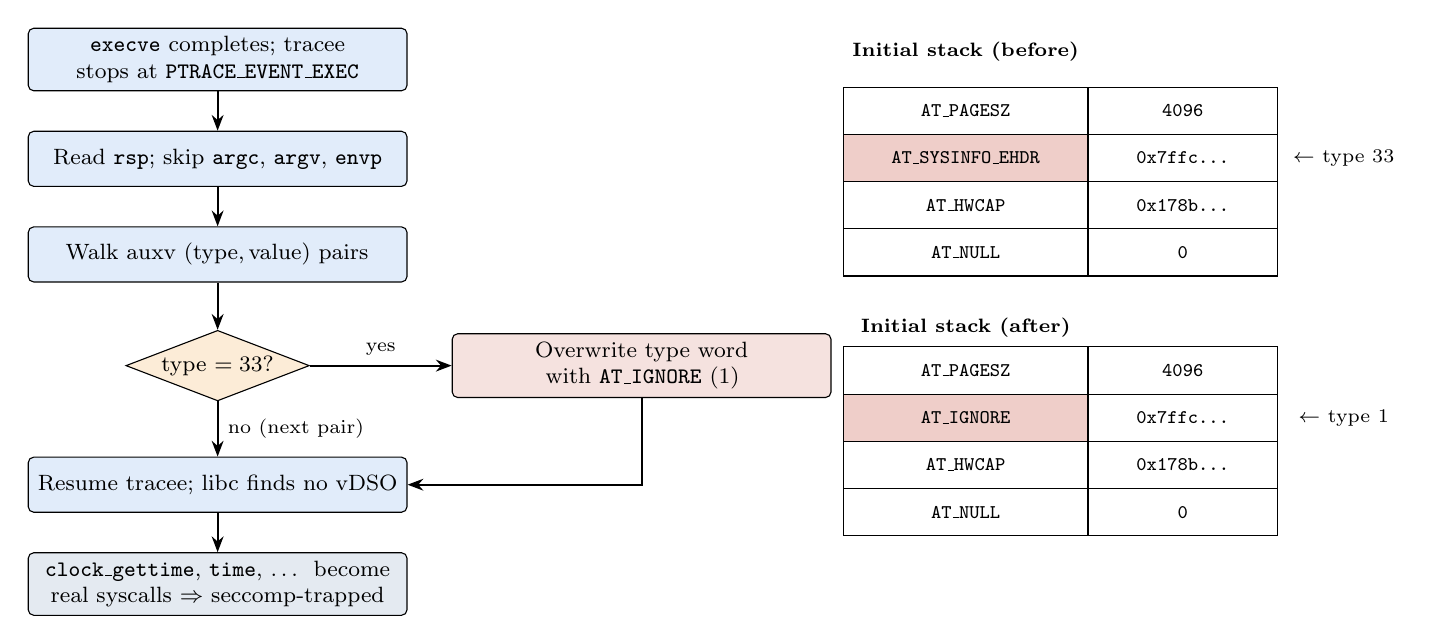
\begin{tikzpicture}[font=\footnotesize,
  node distance=5mm,
  stp/.style={draw,rounded corners=2pt,align=center,fill=supc,minimum height=7mm,text width=4.6cm,inner sep=3pt},
  dec/.style={draw,diamond,aspect=2.6,align=center,fill=chic,inner sep=1pt},
  arr/.style={-{Stealth[length=2mm]},thick},
  cell/.style={draw,minimum width=3.1cm,minimum height=6mm,inner sep=1pt,font=\scriptsize\ttfamily}]
% flowchart
\node[stp] (a) {\texttt{execve} completes; tracee stops at \texttt{PTRACE\_EVENT\_EXEC}};
\node[stp,below=of a] (b) {Read \texttt{rsp}; skip \texttt{argc}, \texttt{argv}, \texttt{envp}};
\node[stp,below=of b] (c) {Walk auxv $(\text{type},\text{value})$ pairs};
\node[dec,below=6mm of c] (d) {type $=33$?};
\node[stp,right=18mm of d,fill=warn!15] (e) {Overwrite type word\\with \texttt{AT\_IGNORE} (1)};
\node[stp,below=7mm of d] (f) {Resume tracee; libc finds no vDSO};
\node[stp,below=of f,fill=accent!12] (g) {\texttt{clock\_gettime}, \texttt{time}, \dots{} become real syscalls $\Rightarrow$ seccomp-trapped};
\draw[arr] (a)--(b); \draw[arr] (b)--(c); \draw[arr] (c)--(d);
\draw[arr] (d)--node[above,font=\scriptsize]{yes}(e);
\draw[arr] (d)--node[right,font=\scriptsize]{no (next pair)}(f);
\draw[arr] (e) |- (f);
\draw[arr] (f)--(g);
% stack before / after
\node[font=\scriptsize\bfseries] at (9.5,0.1) {Initial stack (before)};
\foreach \i/\t/\v in {0/AT\_PAGESZ/4096, 1/AT\_SYSINFO\_EHDR/0x7ffc\ldots, 2/AT\_HWCAP/0x178b\ldots, 3/AT\_NULL/0}{
  \node[cell,fill=white] at (9.5,-0.65-\i*0.6) {\t};
  \node[cell,fill=white,minimum width=2.4cm,anchor=west] at (11.05,-0.65-\i*0.6) {\v};}
\node[cell,fill=warn!25] at (9.5,-1.25) {AT\_SYSINFO\_EHDR};
\node[font=\scriptsize\bfseries] at (9.5,-3.4) {Initial stack (after)};
\foreach \i/\t/\v in {0/AT\_PAGESZ/4096, 1/AT\_IGNORE/0x7ffc\ldots, 2/AT\_HWCAP/0x178b\ldots, 3/AT\_NULL/0}{
  \node[cell,fill=white] at (9.5,-3.95-\i*0.6) {\t};
  \node[cell,fill=white,minimum width=2.4cm,anchor=west] at (11.05,-3.95-\i*0.6) {\v};}
\node[cell,fill=warn!25] at (9.5,-4.55) {AT\_IGNORE};
\node[font=\scriptsize] at (14.3,-1.25) {$\leftarrow$ type 33};
\node[font=\scriptsize] at (14.3,-4.55) {$\leftarrow$ type 1};
\end{tikzpicture}
\caption{Auxiliary-vector scrubbing. Left: the per-\texttt{exec} procedure. Right: the entry for the vDSO has its key changed from 33 to 1; its value is untouched. The same transformation runs at every \texttt{execve} in the process tree.}
\label{fig:auxv}
\end{figure*}

\subsection{Hardware RDTSC emulation}
\label{sec:tsc}
Even with the vDSO gone, \sys{rdtsc} is an unprivileged instruction that reads the cycle counter directly and generates no system call. Linux can make it fault: \sys{prctl(PR_SET_TSC, PR_TSC_SIGSEGV)} causes the instruction to raise \sys{SIGSEGV} in the calling thread~\cite{prctl}. The child enables this before its first instruction; the supervisor, which is the tracer, receives the signal as a signal-delivery stop and does the following.
\begin{enumerate}
\item Read the instruction at \sys{RIP}. Opcode \sys{0F 31} is \sys{rdtsc}; \sys{0F 01 F9} is \sys{rdtscp}. Any other faulting instruction is a genuine crash and is delivered to the program unchanged.
\item Compute the virtual counter $\tau$ from the virtual clock $V$ (in ns) and a nominal frequency $f$ (Hz):
\begin{equation}
\tau(V)=\Big\lfloor \frac{V\cdot f}{10^{9}}\Big\rfloor,\quad
\mathtt{RAX}=\tau \bmod 2^{32},\ \mathtt{RDX}=\tau\gg 32 .
\label{eq:tsc}
\end{equation}
\item For \sys{rdtscp}, also set \sys{RCX} to a virtual core identifier $\pi(\text{tid})$, a deterministic function of the thread, so \sys{rdtscp}-based CPU identification is stable.
\item Advance \sys{RIP} by the instruction length (2 or 3 bytes), suppress the signal, and resume.
\end{enumerate}
Since $\tau$ depends only on $V$, a program that busy-waits on \sys{rdtsc} sees time advance only through the virtual clock's own rules (\S\ref{sec:warp}); it observes neither the host's cycle count nor the speed of the machine.

\subsection{Virtual clock and instant time-warping}
\label{sec:warp}
The virtual clock $V\in\mathbb{N}$ (ns) is monotonic and owned by the supervisor. It advances in two ways: by a fixed cost $c_{\text{sys}}$ per mediated system call, and by $\alpha\,\Delta I$ for each scheduling quantum in which the tracee retired $\Delta I$ instructions (\S\ref{sec:conc}). Both are functions of the program's own execution, not of host speed.

Timed waits do not block. When a thread issues \sys{nanosleep}, \sys{clock_nanosleep}, \sys{epoll_wait} or \sys{poll} with a finite timeout, the supervisor computes the absolute deadline $d=V+\text{timeout}$, inserts the waiter into a min-heap \emph{time wheel} $W$ keyed by $d$, and does not reply to the seccomp notification. Let $R$ be the set of runnable threads. If $R=\emptyset$ the whole tree is idle, and the clock jumps:
\begin{equation}
\Warp:\quad R=\emptyset\ \Longrightarrow\ V \leftarrow \max\Big(V,\ \min_{w\in W} d_w\Big),
\label{eq:warp}
\end{equation}
after which the earliest waiter is released (a sleep returns $0$; an \sys{epoll_wait} with no ready descriptor returns $0$ events). Equation~\eqref{eq:warp} never moves the clock backwards, and it jumps only when nothing can make progress, so the order of all events is the same as in a real-time run; only the idle gaps are removed.

\begin{algorithm}[t]
\caption{Dispatch loop with time warping}
\label{alg:warp}
\While{tree not exited}{
  \If{$R \neq \emptyset$}{
    $t \gets \textsc{PickNext}(R)$ \Comment*[r]{seeded, deterministic order}
    run $t$ for one quantum; $V \mathrel{+}= \alpha\,\Delta I$\;
    \textsc{Handle}(syscall or trap of $t$)\;
  }
  \ElseIf{$W \neq \emptyset$}{
    $w \gets \textsc{PopMin}(W)$;\quad $V \gets \max(V, d_w)$\;
    \textsc{Release}($w$, result $=0$)\;
  }
  \Else{ \textsc{ReportDeadlock}() }
}
\end{algorithm}

The speedup for a sleeping workload of nominal duration $D$ whose supervised wall time is $\varepsilon$ is $S=D/\varepsilon$. For a 10\,s sleep completing in 18\,ms, $S\approx 556\times$; for a 15\,s \sys{epoll_wait} completing in 17\,ms, $S\approx 882\times$ (\S\ref{sec:eval}). The remaining wall time is supervisor overhead (process creation, seccomp installation, dispatch), not waiting.

\subsection{Concurrency, futexes and preemption}
\label{sec:conc}
\paragraph{FutexManager.} Threads block on \sys{futex(FUTEX_WAIT)} and are released by \sys{FUTEX_WAKE}. If these were left to the kernel, wake order would depend on kernel internals. \statis{} instead intercepts them: a userspace \sys{FutexManager} keeps a FIFO wait queue per futex address, parks a waiter by withholding its notification reply, and answers a wake by releasing queued waiters in a fixed order. Futex traffic thus becomes part of the deterministic event stream~\cite{futex}.

\paragraph{Silent thread exit.} \sys{pthread_join} waits on the thread's TID word, which the kernel clears and wakes \emph{by itself} when a thread created with \sys{CLONE_CHILD_CLEARTID} exits. No system call is made by anyone, so the supervisor would never learn the waiter should wake. \statis{} records each thread's \sys{ctid} address at \sys{clone}, observes thread exit through its ptrace exit event, and wakes the \sys{FutexManager} queue for that address itself, restoring a join that would otherwise hang or return in kernel-dependent order.

\paragraph{PMU quanta.} A thread that never calls into the kernel (a spin loop) would starve the others. \statis{} opens a per-thread \sys{perf_event_open} counter of user-mode retired instructions with sample period $Q$; overflow ends the quantum, and the scheduler picks the next runnable thread. The quantum is measured in instructions, not time, so the interleaving is independent of host load, and the seed selects the order in which runnable threads are visited.

\subsection{Deterministic fault injection}
\label{sec:fault}
Reproducing a failure requires failures that are themselves reproducible. Let $k=\mathrm{KDF}(s)$ be a 256-bit key derived from the seed and $n$ the index of the current mediated system call in the deterministic event order. \statis{} draws a word from ChaCha20~\cite{chacha}:
\begin{equation}
u_n=\frac{\mathrm{ChaCha20}_{k}(n)}{2^{32}},\qquad
\text{inject}\iff u_n<p_c\ \wedge\ \text{fd}>2,
\label{eq:fault}
\end{equation}
where $p_c$ is the configured probability for the call's class $c$. The error is selected from a class-specific set using a second word of the same stream: network operations draw from \{\sys{-ECONNRESET}, \sys{-ETIMEDOUT}\}, nonblocking I/O from \{\sys{-EAGAIN}\}, and blocking calls may also see \sys{-EINTR} or \sys{-EIO}. File descriptors $\le 2$ (stdin, stdout, stderr) are \emph{protected}: errors injected there would corrupt the program's output channel and the supervisor's own diagnostics rather than test its logic. Because $n$ is a position in a deterministic order, the same seed reproduces the same failure at the same call.

\subsection{Process hierarchy and virtual PIDs}
\label{sec:pid}
Real PIDs vary from run to run, so a program that prints or hashes its PID is nondeterministic. \statis{} presents a synthetic hierarchy: \sys{getpid} returns 1000, \sys{getppid} returns 999, and \sys{gettid} returns a stable per-thread virtual identifier assigned in creation order. Signals are the inverse problem: \sys{SYS_kill} and \sys{SYS_tgkill} carry virtual identifiers, which the supervisor maps to the corresponding \emph{real} OS PIDs before performing the call, so a program signalling its ``parent'' or a sibling reaches the right target.

\subsection{Compact trace and semantic replay}
\label{sec:trace}
Because the seed determines the schedule, time, and faults, \statis{} does not need to store inputs to \emph{reproduce} a run; the trace's role is to \emph{verify} that a re-execution has not diverged, and to support debugging. The trace is a little-endian binary stream: a header (magic, version, seed, configuration) followed by one fixed-layout record per mediated event holding thread id, syscall number, a small vector of \emph{semantic} argument digests, and the result. Its size grows with the number of events, not with the bytes the program moves, and so is measured in kilobytes where \sys{rr} recordings, which capture memory and I/O contents, reach gigabytes~\cite{rr}.

\paragraph{Semantic matching.} Raw argument words are not stable across runs even when behavior is: a different environment size or ASLR slide shifts stack pointers, so a pointer to a buffer in a \sys{read} has a different value each run. Comparing raw words would flag a divergence on every event. Replay therefore compares a normalized form: file descriptors and flags by value, lengths by value, string arguments (paths) by content, and pointer arguments are \emph{ignored}. Two events match iff
\begin{equation}
(\text{tid},\ \text{nr},\ \sigma(\mathbf{a}),\ \text{ret})=(\text{tid}',\ \text{nr}',\ \sigma(\mathbf{a}'),\ \text{ret}'),
\label{eq:semantic}
\end{equation}
where $\sigma$ projects the argument vector to its semantic components. The first mismatch is reported with its event index.

%=========================================================================
\section{Implementation}
%=========================================================================
\statis{} targets Linux on x86-64, because \sys{PR_SET_TSC} and the \sys{rdtsc} decoding are x86-specific. It requires no kernel module or root privilege beyond what \sys{ptrace}, seccomp user notification (\sys{seccomp_unotify}~\cite{unotify}) and \sys{perf_event_open}~\cite{perf} need. The supervisor is a single process: a ptrace event loop plus the notification loop. Dispatch is table-driven by syscall number, and each mediated class (time, sleep/poll, futex, identity, signal, I/O) has its own handler. Handlers that must act on the tracee's memory (strings for the trace, \sys{timespec} arguments) read it from the tracee's address space. \pending{source line counts, language, build and dependency footprint from the repository}

%=========================================================================
\section{Evaluation}
\label{sec:eval}
%=========================================================================
\paragraph{Setup.} \pending{host CPU, kernel version, virtualization, PMU availability, number of runs, how wall time is measured.} All time-warp numbers below are wall-clock times of the supervised process tree, from launch to exit.

\subsection{Comparison with related systems}
Table~\ref{tab:compare} compares \statis{} with native Linux and the three systems closest in goal. Entries for other systems follow their public documentation and papers; we mark those that deserve checking against current releases.

\begin{table*}[t]
\centering
\small
\caption{Competitive comparison. $\dagger$: from public documentation; behaviour may differ across versions. ``Seed'' means a user-chosen integer selects the schedule.}
\label{tab:compare}
\begin{tabular}{@{}l c c c c c@{}}
\toprule
 & Native Linux & Mozilla \texttt{rr}~\cite{rr} & Meta \texttt{Hermit}~\cite{hermit} & DetTrace~\cite{dettrace} & \statis{} \\
\midrule
Runs unmodified binaries & \yes & \yes & \yes & \yes & \yes \\
No kernel changes & \yes & \yes & \yes$^\dagger$ & \yes$^\dagger$ & \yes \\
Deterministic re-execution & \no & replay of a recording & \yes & \yes & \yes (seed) \\
Seeded schedule exploration & \no & chaos mode$^\dagger$ & \yes$^\dagger$ & \no$^\dagger$ & \yes \\
Idle-wait time warp (sleep/poll/epoll) & \no & \no & partial$^\dagger$ & \no$^\dagger$ & \yes \\
Seeded syscall error injection & \no & \no & \no$^\dagger$ & \no$^\dagger$ & \yes \\
Replay artifact & none & full recording (GB) & seed$^\dagger$ & re-execution$^\dagger$ & seed + trace (KB) \\
\bottomrule
\end{tabular}
\end{table*}

\subsection{Time warping}
Figure~\ref{fig:warp} shows the headline result. A process that sleeps for 10\,s completes in 18\,ms under \statis{}, and one that blocks 15\,s in \sys{epoll_wait} with no ready descriptor completes in 17\,ms: speedups of roughly $556\times$ and $882\times$, both above the $500\times$ mark. A test suite dominated by timeouts, retries and heartbeats can therefore be run in a small fraction of its nominal duration while seeing the same event order.

\begin{figure}[t]
\centering
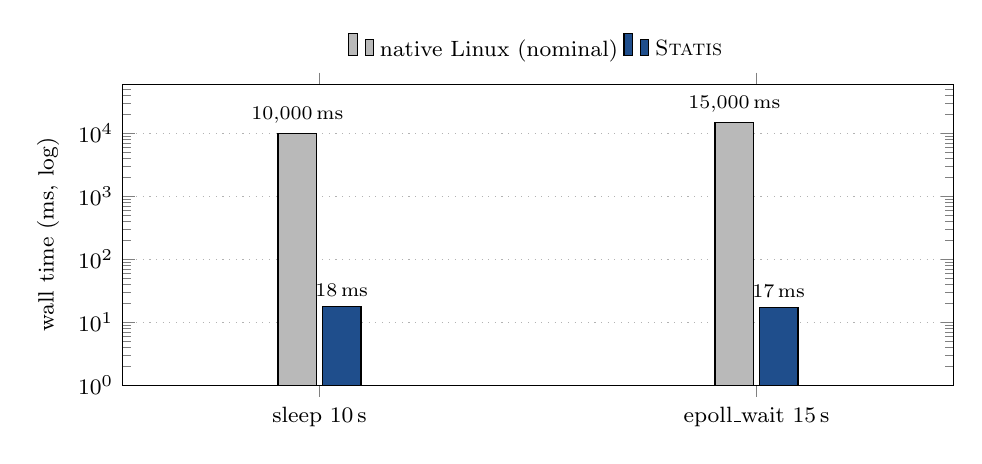
\begin{tikzpicture}
\begin{axis}[
  ybar, bar width=14pt,
  width=\columnwidth, height=5.4cm,
  ymode=log, ymin=1, ymax=60000,
  ylabel={wall time (ms, log)},
  symbolic x coords={sleep 10\,s, epoll\_wait 15\,s},
  xtick=data, enlarge x limits=0.45,
  legend style={at={(0.5,1.04)},anchor=south,legend columns=2,font=\footnotesize,draw=none},
  nodes near coords, point meta=explicit symbolic,
  every node near coord/.append style={font=\scriptsize},
  tick label style={font=\footnotesize}, label style={font=\footnotesize},
  ymajorgrids, grid style={dotted,gray!60}]
\addplot[fill=gray!55,draw=black] coordinates {(sleep 10\,s,10000) [10{,}000\,ms] (epoll\_wait 15\,s,15000) [15{,}000\,ms]};
\addplot[fill=accent,draw=black] coordinates {(sleep 10\,s,18) [18\,ms] (epoll\_wait 15\,s,17) [17\,ms]};
\legend{native Linux (nominal), \statis{}}
\end{axis}
\end{tikzpicture}
\caption{Time-warp speedup (log scale). \statis{} completes a 10\,s sleep in 18\,ms ($\approx$556$\times$) and a 15\,s \texttt{epoll\_wait} in 17\,ms ($\approx$882$\times$). Native values are the nominal durations.}
\label{fig:warp}
\end{figure}

\subsection{Trace storage}
Figure~\ref{fig:trace} contrasts the artifact needed to replay a run. \texttt{rr} stores a recording that includes the contents of nondeterministic inputs and grows to gigabytes; \statis{} stores only event records, in kilobytes, because the seed regenerates the rest.

\begin{figure}[t]
\centering
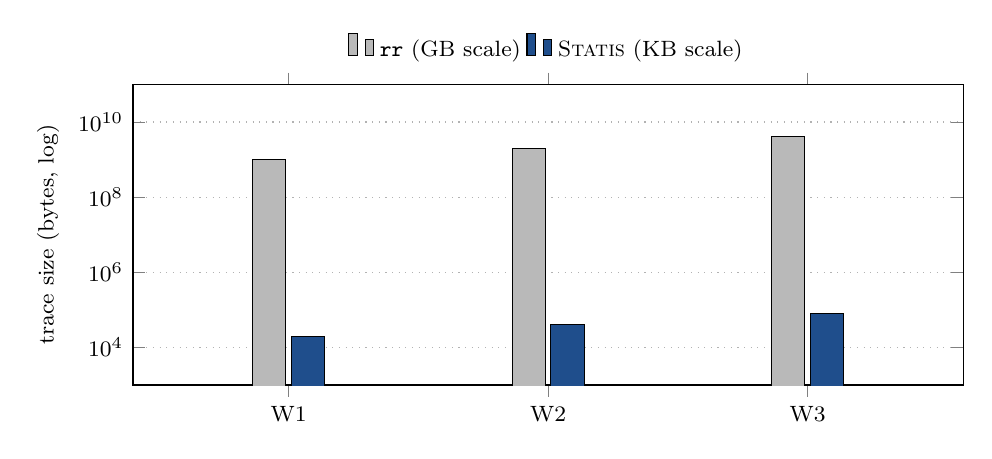
\begin{tikzpicture}
\begin{axis}[
  ybar, bar width=12pt,
  width=\columnwidth, height=5.4cm,
  ymode=log, ymin=1e3, ymax=1e11,
  ylabel={trace size (bytes, log)},
  symbolic x coords={W1,W2,W3},
  xtick=data, enlarge x limits=0.3,
  legend style={at={(0.5,1.04)},anchor=south,legend columns=2,font=\footnotesize,draw=none},
  tick label style={font=\footnotesize}, label style={font=\footnotesize},
  ymajorgrids, grid style={dotted,gray!60}]
% PLACEHOLDER VALUES: replace with measured sizes. rr ~ GB scale, statis ~ KB scale.
\addplot[fill=gray!55,draw=black] coordinates {(W1,1e9) (W2,2e9) (W3,4e9)};
\addplot[fill=accent,draw=black] coordinates {(W1,2e4) (W2,4e4) (W3,8e4)};
\legend{\texttt{rr} (GB scale), \statis{} (KB scale)}
\end{axis}
\end{tikzpicture}
\caption{Trace storage, \texttt{rr} vs.\ \statis{}. \pending{plotted values are layout placeholders at the stated orders of magnitude (GB vs.\ KB); replace with measured sizes for named workloads W1--W3}.}
\label{fig:trace}
\end{figure}

\subsection{Microbenchmarks}
Table~\ref{tab:micro} reports per-operation costs. Only the two time-warp rows are measured so far.

\begin{table}[t]
\centering
\small
\caption{Microbenchmarks. Wall time is for the whole supervised process.}
\label{tab:micro}
\begin{tabular}{@{}l r r r@{}}
\toprule
Target & Native & \statis{} & Speedup \\
\midrule
\sys{nanosleep} 10\,s & 10{,}000\,ms & 18\,ms & 556$\times$ \\
\sys{epoll_wait} 15\,s & 15{,}000\,ms & 17\,ms & 882$\times$ \\
\sys{clock_gettime} latency & \pending{} & \pending{} & --- \\
\sys{rdtsc} trap latency & \pending{} & \pending{} & --- \\
\sys{pthread} create+join & \pending{} & \pending{} & --- \\
Mediated syscall (\sys{getpid}) & \pending{} & \pending{} & --- \\
Fault-injection overhead & \pending{} & \pending{} & --- \\
Trace write throughput & \pending{} & \pending{} & --- \\
\bottomrule
\end{tabular}
\end{table}

\subsection{Determinism check}
\pending{$N$ repeated runs per seed on a suite including multithreaded and multi-\sys{exec} programs; report the fraction with identical traces, and the effect of changing environment size on semantic vs.\ raw matching.}

%=========================================================================
\section{Related Work}
%=========================================================================
\paragraph{Record and replay.} \texttt{rr}~\cite{rr} records a run on one machine and replays it with full debugger support, using ptrace, seccomp-bpf and hardware performance counters. Its recordings capture input data and are large; \statis{} trades that universality for a seed and a small trace.

\paragraph{Deterministic containers and execution.} DetTrace~\cite{dettrace} runs programs in a container that removes sources of nondeterminism, for reproducible builds. Hermit~\cite{hermit}, built on the Reverie interposition framework~\cite{reverie}, adds a deterministic scheduler, virtual time and a seed-driven chaos mode. \statis{} is closest in spirit; it differs in its combination of per-exec auxv scrubbing, \sys{PR_TSC_SIGSEGV} emulation, an explicit time wheel that warps idle trees, seeded error injection and a semantic-matching trace. Earlier work obtains determinism by changing the OS or runtime: Determinator~\cite{determinator}, or by instrumenting multithreaded programs: Kendo~\cite{kendo}, CoreDet~\cite{coredet}, Dthreads~\cite{dthreads}.

\paragraph{Virtual time and simulation.} Shadow~\cite{shadow} runs real network applications under a discrete-event simulated clock; FoundationDB's deterministic simulation~\cite{fdb} finds distributed-systems bugs by running under a seeded simulator. \statis{} brings virtual time and seeded faults to arbitrary unmodified binaries rather than to a purpose-built simulator.

%=========================================================================
\section{Limitations}
\label{sec:limits}
%=========================================================================
\begin{itemize}
\item \textbf{Closed world.} Determinism holds for the supervised tree. Nondeterminism that enters from outside (real network peers, other host processes, shared files modified concurrently) is outside the contract; time warping is only sound when no external event can make an idle tree runnable.
\item \textbf{Architecture.} The \sys{rdtsc} path is x86-specific; other ISAs need their own counter emulation.
\item \textbf{PMU dependence.} Instruction-quantum preemption needs a usable performance counter; some virtual machines hide it, and counter skid limits how exactly a quantum boundary is placed. \pending{fallback behaviour and its determinism guarantees}
\item \textbf{Overhead.} Each mediated syscall is a supervisor round trip. \pending{measured per-syscall overhead on syscall-heavy workloads}
\item \textbf{Scope of evidence.} Only the two time-warp results are measured in this draft; the trace-size comparison is at order-of-magnitude level, and the benchmark suite, determinism-rate study and baselines on equal workloads are pending.
\end{itemize}

%=========================================================================
\section{Conclusion}
%=========================================================================
Nondeterminism in a Linux program enters through a short list of doors. Close them all from userspace---blind the vDSO at every \sys{exec}, trap the cycle counter, warp idle time, order futexes and quanta by seed, derive errors from the same seed---and an unmodified binary becomes a function of one integer. In that regime a 10\,s sleep costs 18\,ms, and a replay artifact is kilobytes rather than gigabytes. The next steps are the full evaluation listed above and a fused fast path for the hottest system calls.

%=========================================================================
\begin{thebibliography}{99}\small
\bibitem{rr} R.~O'Callahan, C.~Jones, N.~Froyd, K.~Huey, A.~Noll, N.~Partush. Engineering record and replay for deployability. In \emph{USENIX ATC}, 2017.
\bibitem{dettrace} O.~Navarro Leija, K.~Shiptoski, R.~G.~Scott, B.~Wang, N.~Renner, R.~R.~Newton, J.~Devietti. Reproducible containers. In \emph{ASPLOS}, 2020.
\bibitem{hermit} Meta Platforms. Hermit: a hermetic, deterministic Linux sandbox. \url{https://github.com/facebookexperimental/hermit}, 2022.
\bibitem{reverie} Meta Platforms. Reverie: a user-space system-call interception framework. \url{https://github.com/facebookexperimental/reverie}.
\bibitem{determinator} A.~Aviram, S.-C.~Weng, S.~Hu, B.~Ford. Efficient system-enforced deterministic parallelism. In \emph{OSDI}, 2010.
\bibitem{kendo} M.~Olszewski, J.~Ansel, S.~Amarasinghe. Kendo: efficient deterministic multithreading in software. In \emph{ASPLOS}, 2009.
\bibitem{coredet} T.~Bergan, O.~Anderson, J.~Devietti, L.~Ceze, D.~Grossman. CoreDet: a compiler and runtime system for deterministic multithreaded execution. In \emph{ASPLOS}, 2010.
\bibitem{dthreads} T.~Liu, C.~Curtsinger, E.~D.~Berger. Dthreads: efficient deterministic multithreading. In \emph{SOSP}, 2011.
\bibitem{shadow} R.~Jansen, N.~Hopper. Shadow: running Tor in a box for accurate and efficient experimentation. In \emph{NDSS}, 2012.
\bibitem{fdb} J.~Zhou et al. FoundationDB: a distributed unbundled transactional key value database. In \emph{SIGMOD}, 2021.
\bibitem{futex} H.~Franke, R.~Russell, M.~Kirkwood. Fuss, futexes and furwocks: fast userlevel locking in Linux. In \emph{Ottawa Linux Symposium}, 2002.
\bibitem{chacha} D.~J.~Bernstein. ChaCha, a variant of Salsa20. In \emph{SASC}, 2008. See also Y.~Nir, A.~Langley, RFC 8439, 2018.
\bibitem{vdso} Linux man-pages. \emph{vdso(7)} and \emph{getauxval(3)}.
\bibitem{prctl} Linux man-pages. \emph{prctl(2)}, \texttt{PR\_SET\_TSC}; and \emph{ptrace(2)}.
\bibitem{unotify} Linux man-pages. \emph{seccomp\_unotify(2)}.
\bibitem{perf} Linux man-pages. \emph{perf\_event\_open(2)}.
\end{thebibliography}

\end{document}
